\begin{figure}[h!]
     \centering
    \captionsetup[sub]{font=small}
     \begin{subfigure}[b!]{0.44 \textwidth}
         \caption{}
         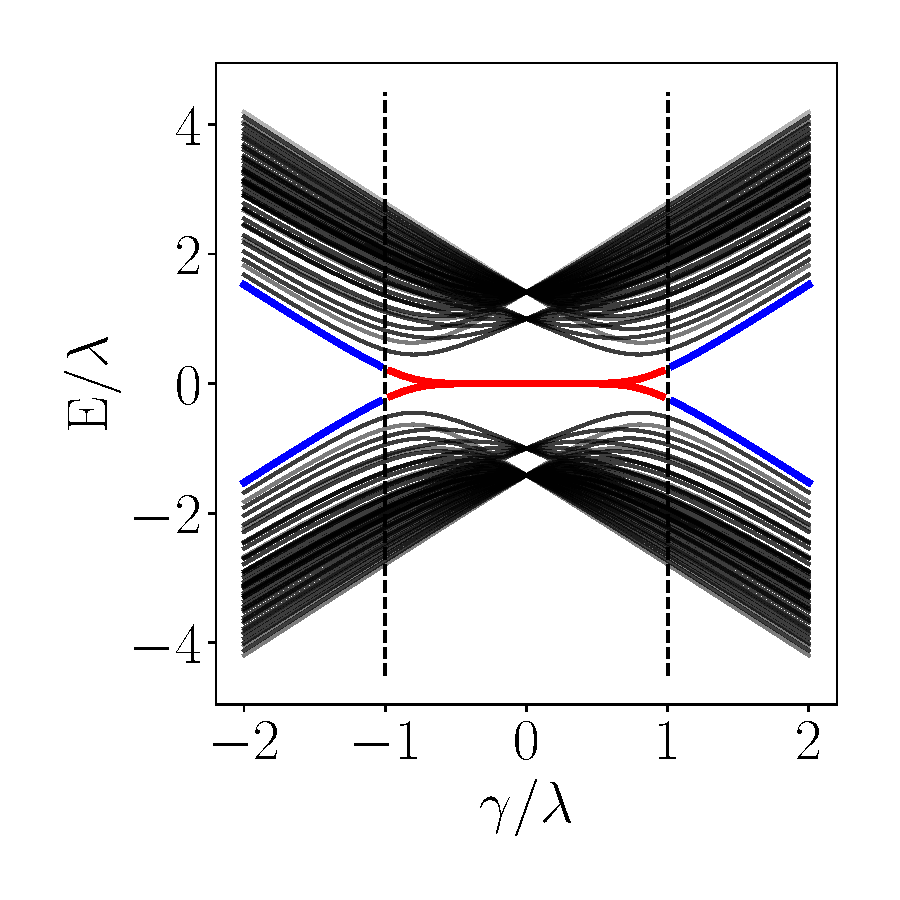
\includegraphics[width=\textwidth]{Imagenes/Resultados_Hoti_Cuadrado/bands_square_shh.pdf}
     \end{subfigure}\hspace*{1em}
     \begin{subfigure}[b!]{0.56 \textwidth}
         \caption{}
         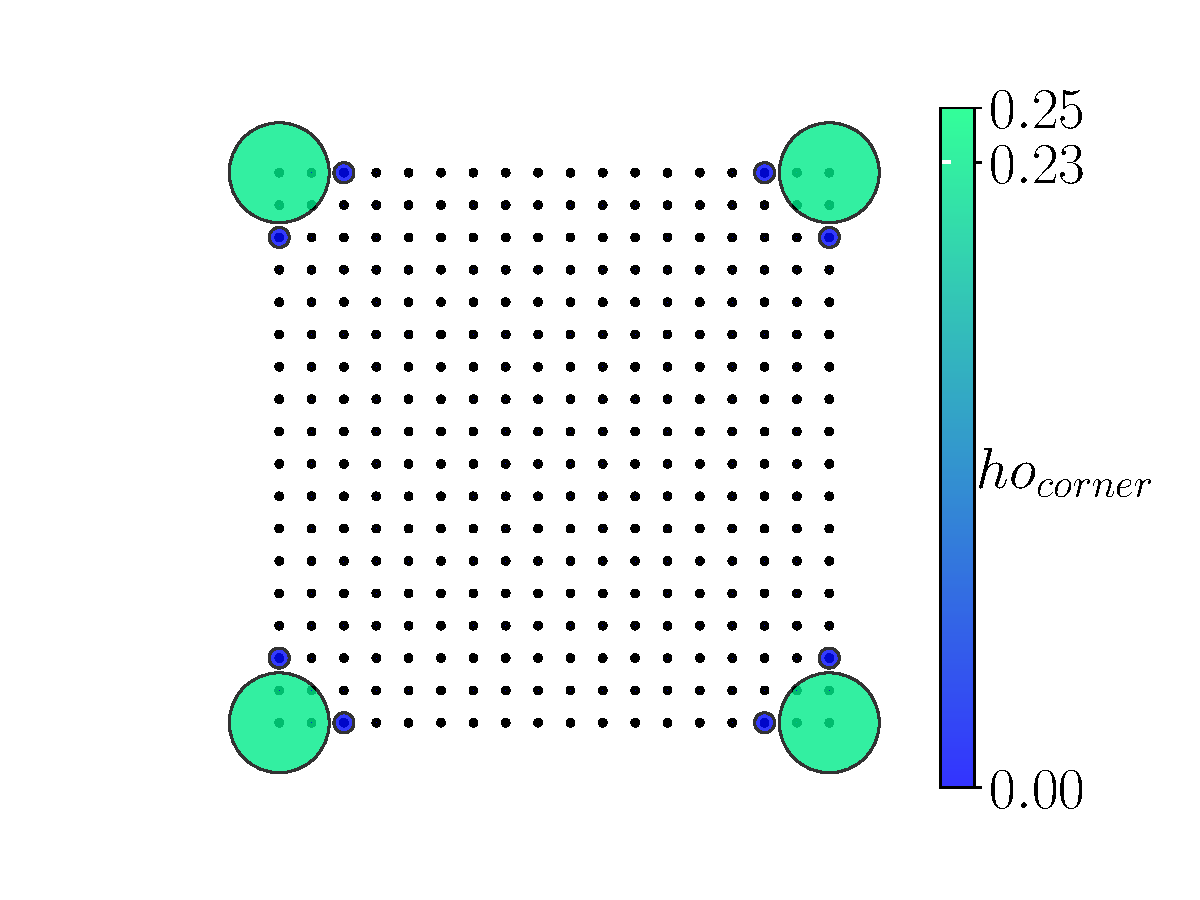
\includegraphics[width=\textwidth]{Imagenes/Resultados_Hoti_Cuadrado/proyection_square.pdf}
     \end{subfigure}\hspace*{1em} \vspace*{-0.5em}
        \caption{\textbf{a)}Espectro de energía del sistema con geometría cuadrada y condiciones abiertas a la frontera, como función de $\gamma/\lambda$. Las energías centrales coloreadas en rojo corresponde a los 4 estados localizados en las esquinas. \textbf{b)} Densidad de probabilidad en un fase no trivial donde $\gamma = 1,\, \, \lambda = 4.5$, en un red cuadrada de $18\times18$ sitios.}
    \label{fig:Pram_Proy_cuadrado}
\end{figure}